\documentclass{book}
\usepackage[utf8]{inputenc}
\usepackage{natbib}
\usepackage{xcolor}
\usepackage{graphicx}
\usepackage{fancyhdr}
\usepackage[T1]{fontenc}    % use 8-bit T1 fonts
\usepackage[colorlinks = true,
            linkcolor = blue,
            urlcolor  = blue,
            citecolor = blue,
            anchorcolor = blue]{hyperref}
\usepackage{url}            % simple URL typesetting
\usepackage{booktabs}       % professional-quality tables
\usepackage{amsfonts}       % blackboard math symbols
\usepackage{nicefrac}       % compact symbols for 1/2, etc.
\usepackage{microtype}      % microtypography
\usepackage{lipsum}
\usepackage[margin=1in]{geometry}
\usepackage{amsmath}
\usepackage{subcaption}
\usepackage{tabularx}

\renewcommand\cfoot{\page}

\title{\emph{Brief} Spring 2019 Review}
\author{Jalen Cates}
\date{April 2019}

\begin{document}

\maketitle

\vspace*{25pt}
\Large{\emph{Disclaimer:} These are what I am personally making for my review, so I make no guarantee this is helpful, complete, or anything. Please tell me if anything is false on it or should be added. Good luck!}
\normalsize


\tableofcontents


\chapter{Thermal Physics Before the Midterm}

\section{Kittel \& Kroemer: Chapter 1 and 2}
Derives statistical mechanics from the fundamental assumption. The assumption is: \emph{Every particular state of a system is occupied with equal probability}. The number of available states with a given energy implies the maximum entropy principle. 
\begin{itemize}
    \item Accessible states: $g(N,U)$
    \item For multiple systems put together: $g = g_1 \cdot ... \cdot g_n$
    \item Entropy: $S=k_B \sigma = k_B \log{g}$
    \item Temperature: $\tau = k_B T = (\partial U/ \partial \sigma)_{N,V}$
\end{itemize}


\section{Callen: Chapter 1}
Goes over the very basics and tries to build an intuitive relationship between energy and entropy and other extensive parameters.
\begin{itemize}
    \item \textbf{Postulate I.} \emph{There exist particular states (called equilibrium states) of simple systems that, macroscopically, are characterized completely by internal energy U, the volume V, and the mole numbers N.}
    \item \textbf{Postulate II.} \emph{There exists a function (called the entropy S) of the extensive parameters of any composite system, defined for all equilibrium states and having the following property: The values assumed by the extensive parameters in the absence of an internal constraint are those that maximize the entropy over the manifold of constrained equilibrium states.}
    \item \textbf{Postulate III.} \emph{The entropy of a composite system is additive over the constituent subsystems. The entropy is continuous and differentiable and is a monotonically increasing function of energy.}
    \item \textbf{Postulate IV.} \emph{The entropy of any system vanishes in the state of zero temperature.}
\end{itemize}

Work and Heat: $dU = dQ + dW_M = TdS - PdV$

\section{Callen: Chapter 2}

Intensive parameters are those given by the partial derivatives of the fundamental relation. They are defined by the following:

\begin{align*}
    (\partial U/\partial S)_{V,N} & \equiv  T & (\partial S/\partial U)_{V,N} & \equiv  1/T \\ 
    (\partial U/\partial V)_{S,N} & \equiv -P & (\partial S/\partial V)_{U,N} & \equiv -P/T \\ 
    (\partial U/\partial N)_{S,V} & \equiv \mu & (\partial S/\partial N)_{U,V} & \equiv \mu/T
\end{align*}
\begin{equation}
    dU = TdS-PdV+\mu dN
\end{equation}
\begin{equation}
    dS = \frac{1}{T} dU + \frac{P}{T} dV - \frac{\mu}{T} dN
\end{equation}
The chapter also goes over the conditions for equilibrium with heat flow, mechanical equilibrium, and equilibrium with matter flow. These are rather straightforward to derive, so they are omitted. (\emph{Note: Stoichiometry is important when dealing with chemical equilibrium.})

\section{Callen: Chapter 3}
Goes over Euler and Gibbs-Duhem relation then summarizes information about the fundamental relation. The chapter then covers ideal gases, Van der Waals fluid, radiation, and the rubber band. The last section goes over the preferred derivatives briefly ($\alpha, c_p, \kappa_T$).
\begin{itemize}
    \item Euler Relation: $U=TS-PV+\mu N$
    \item Gibbs-Duhem Relation: relations among the derivatives of U. The one for single-component system is $0 = S dT - V dP + N d\mu $
    \item The fundamental relation contains all information about a thermodynamic system.
    \item Two equations of state [such as T,P] can determine the fundamental relation with an unknown constant using the Gibbs-Duhem relation.
    \item NOTE: The potentials given by Legendre Transformations are not fundamental relations!
\end{itemize}


\section{Callen: Chapter 4}
Covers possible processes, quasi-static processes, reversible processes, maximum work theorem, Carnot cycle, refrigeration, and Otto cycle.

\begin{itemize}
    \item A process is possible if and only if $\Delta S \geq 0$ and the laws of mechanics are obeyed.
    \item Quasi-Static Process: idealized process where each state can be represented with the fundamental relation as an equilibrium state.
    \item There is a relaxation time $\tau$ between equilibrium states, which is the limit for a process to be \emph{quasi-static}. (Usually related to the speed of sound.)
    \item Reversible Process: $\delta S_{Total}=0$ \emph{Note: Subsystems must still maximize entropy.}
    \item Maximum Work Theorem: reversible process with work extracted from the heat transferred between subsystems
    \item See \emph{Figure 4.6} on page 115 for diagrams of engine, refrigerator, and heat pump.
\end{itemize}

\textbf{Carnot Cycle:}\footnote{I suggest googling this and reading wikipedia or another source.} A hot reservoir and cold reservoir are put into contact with a reversible work source. The following cycle is done:

\begin{enumerate}
    \item Isothermal expansion
    \item Isentropic (reversible adiabatic) expansion
    \item Isothermal compression
    \item Adiabatic reversible compression
\end{enumerate}
\begin{figure}[h]
    \centering
    \begin{minipage}{.5\textwidth}
      \centering
      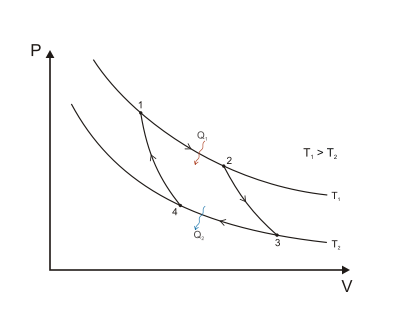
\includegraphics[width=.6\linewidth]{Images/Carnot_P-V.png}
      \captionof{figure}{Carnot Cycle Pressure-Volume Plot}
      \label{fig:test1}
    \end{minipage}%
    \begin{minipage}{.5\textwidth}
      \centering
      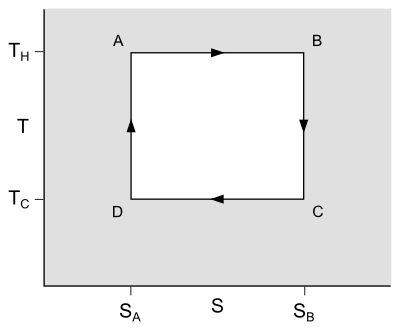
\includegraphics[width=.6\linewidth]{Images/Carnot_T-S.png}
      \captionof{figure}{Carnot Cycle Temperature-Entropy Plot}
      \label{fig:test2}
    \end{minipage}
\end{figure}
\begin{center}
\rule{.8\textwidth}{.5pt}
\end{center}
\textbf{Otto Cycle:} Idealized cycle of a typical spark ignition piston engine often used in automobile engines. The following image sums it up:
\begin{figure}[ht]
    \centering
    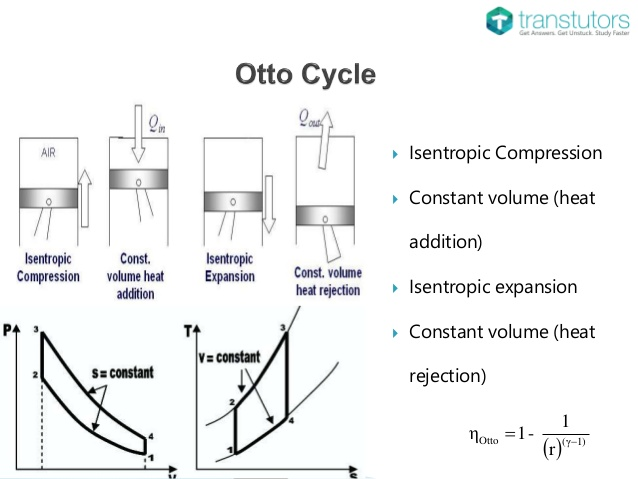
\includegraphics[scale=.4]{Images/otto-cycle.jpg}
    \caption{Otto Cycle Summary}
    \label{fig:otto}
\end{figure}

\section{Callen: Chapter 5}
Covers the Energy Minimum Principle, Legendre Transformations, and the resulting potentials. These are developed because experimentation usually finds the intensive parameters easier to measure. The book also briefly goes over Massieu Functions (Legendre Transformations of the entropy), but this was not covered in class.

\textbf{Energy Minimum Principle:} The Entropy Maximum Principle implies a corollary principle for the minimization of internal energy in a system.

\textbf{Legendre Transformations:} The process replaces a number of the function's variables with the partial derivatives in those variables. 

\begin{center}
    \rule{.8\textwidth}{.5pt}
    
    \textbf{Helmholtz Potential or Free Energy}
    
    $F \equiv U - TS \implies dF = -SdT - PdV + \mu_1dN_1 + \mu_2dN_2 + ... $
    \rule{.8\textwidth}{.5pt}
\end{center}
\begin{tabularx}{\textwidth}{X | X}
    {\begin{align*}
        & U = U(S,V,N_1,N_2,...) \\
        & T = \partial U/\partial S \\
        & F = U - TS \\
        & \text{Elimination of U and S} \\
        & F = F(T,V,N_1,N_2,...)
    \end{align*}} 
    & 
    {\begin{align*}
        & F=F(T,V,N_1,N_2,...) \\
        & -S = \partial F/\partial T \\
        & U = F + TS \\
        & \text{Elimination of F and T} \\
        & U = U(S,V,N_1,N_2,...)
    \end{align*}} 
\end{tabularx}
\begin{center}
    \rule{.8\textwidth}{.5pt}
    
    \textbf{Enthalpy}
    
    $H \equiv U + PV \implies dH = TdS + VdP + \mu_1dN_1 + \mu_2dN_2 + ... $
    \rule{.8\textwidth}{.5pt}
\end{center}
\begin{tabularx}{\textwidth}{X | X}
    {\begin{align*}
        & U = U(S,V,N_1,N_2,...) \\
        & -P = \partial U/\partial V \\
        & H = U + PV \\
        & \text{Elimination of U and V} \\
        & H = H(S,P,N_1,N_2,...)
    \end{align*}} 
    & 
    {\begin{align*}
        & H=H(S,P,N_1,N_2,...) \\
        & V = \partial H/\partial P \\
        & U = H - PV \\
        & \text{Elimination of H and P} \\
        & U = U(S,V,N_1,N_2,...)
    \end{align*}} 
\end{tabularx}
\begin{center}
    \rule{.8\textwidth}{.5pt}
    
    \textbf{Gibbs Potential or Free Energy}
    
    $G \equiv U - TS + PV \implies dG = -SdT + VdP + \mu_1dN_1 + \mu_2dN_2 + ... $
    \rule{.8\textwidth}{.5pt}
\end{center}
\begin{tabularx}{\textwidth}{X | X}
    {\begin{align*}
        & U = U(S,V,N_1,N_2,...) \\
        & T = \partial U/\partial S \\
        & -P = \partial U/\partial V \\
        & G = U - TS + PV \\
        & \text{Elimination of U, V, and S} \\
        & G = G(T,P,N_1,N_2,...)
    \end{align*}} 
    & 
    {\begin{align*}
        & G=G(T,P,N_1,N_2,...) \\
        & -S = \partial G/\partial T \\
        & V = \partial G/\partial P \\
        & U = G + TS - PV \\
        & \text{Elimination of G, P, and T} \\
        & U = U(S,V,N_1,N_2,...)
    \end{align*}} 
\end{tabularx}
\newpage
\begin{center}
    \rule{.8\textwidth}{.5pt}
    
    \textbf{Grand-Canonical Potential}
    
    $U[T,\mu] \equiv U - TS - \mu N \implies dU = -SdT - PdV - Nd\mu$
    \rule{.8\textwidth}{.5pt}
\end{center}
\begin{tabularx}{\textwidth}{X | X}
    {\begin{align*}
        & U = U(S,V,N_1,N_2,...) \\
        & T = \partial U/\partial S \\
        & \mu = \partial U/\partial N \\
        & U[T,\mu] = U - TS - \mu N \\
        & \text{Elimination of U, N, and S} \\
        & U = U(T,P,\mu)
    \end{align*}} 
    & 
    {\begin{align*}
        & U = U(T,P,\mu) \\
        & -S = \partial U[T,\mu]/\partial T \\
        & -N = \partial U[T,\mu]/\partial \mu \\
        & U = U[T,\mu] + TS + \mu N \\
        & \text{Elimination of G, P, and T} \\
        & U = U(S,V,N)
    \end{align*}} 
\end{tabularx}



\section{Processes in Systems}

\begin{table}[!htbp]
    \caption{Types of Processes}
    \centering
        \begin{tabular}{c|c c}
            \toprule
            Name        & Meaning                  & Notes \\
            \midrule
            Adiabatic   & $\Delta N,\Delta Q = 0$  & \\
            Isobaric    & $\Delta P = 0$           & \\
            Isochoric   & $\Delta V = 0$           & \\
            Isothermal  & $\Delta T = 0$           & \\
            Isentropic  & $\Delta N, \Delta Q = 0$ & Also reversible \\
            Isenthalpic & $\Delta H = 0$           &
    \end{tabular}
    \label{tab:processes}
\end{table}


\chapter{Thermal Physics Through the Final}

\section{Main Potentials}

\emph{Know these and when to use them. See Callen chapter 5 on Legendre Transformations.}

\textbf{General Minimum Principle for Legendre Transforms:} The equilibrium value of any unconstrained internal parameter in a system in contact with a set of reservoirs (with intensive parameters $P_1^r,P_2^r,...$) minimizes the thermodynamic potential $U[P_1,P_2,...]$ at constant $P_1,P_2,...$ equal to the reservoir values of that parameter.

\begin{table}[!htbp]
    \caption{Four Main Potentials}
    \centering
        \begin{tabular}{c|c c c}
            \toprule
            Name       & Symbol & Independent Variables  & When? \\
            \midrule
            Energy     & U      & S,V,N                  &  \\
            Helmholtz  & F      & T,V,N                  & Const. T \\
            Enthalpy   & H      & S,P,N                  & Const. P\\
            Gibbs      & G      & T,P,N                  & Const. T,P
    \end{tabular}
    \label{tab:4Potentials}
\end{table}


\section{Energy Minimum Principles}

\emph{Callen: Chapter 6}
\begin{itemize}
    \item Know when to use each potential
\end{itemize}
One of the primary advantages of Legendre Transformations is the elimination of extensive parameters based on the system setup.

\begin{table}[!htbp]
    \caption{Energy Minimum For Legendre Transforms}
    \centering
        \begin{tabular}{c|c c p{5cm}}
            \toprule
            Name       & Reservoir & Minimized Cond. & Usage  \\
            \midrule
            Helmholtz  & $T_r$       & $T_{sys} = T_r$   & Many systems can be approximated as being in contact with the temperature reservoir of its surroundings. \\
            \midrule
            Enthalpy   & $P_r$       & $P_{sys} = P_r$   & Most systems have the atmospheric pressure as a reservoir but also ambient temperature, so the Gibbs is more useful in general. \\
            \midrule
            Gibbs      & $P_r,T_r$   & $P_{sys} = P_r, T_{sys} = T_r$  & This is the situation of most experiments in contact with the atmosphere.
    \end{tabular}
    \label{tab:minimum}
\end{table}
\section{Canonical Formalism}

\emph{Kittel \& Kroemer: Chapter 3}
\begin{itemize}
    \item Thermal reservoir
    \item Weighting of states
    \item When to use Canonical Formalism 
    \item How to make partition function
    \item How to use partition function to get expectation values
\end{itemize}

\subsection{Summary of Chapter}
Consists of lots of definitions and derivations of thermal we learned in Callen.

\textbf{Boltzmann Factor: } $e^{-\epsilon/\tau}$ gives the relative probability of a given configuration with energy $\epsilon$.

\textbf{Partition Function (Z): } The sum of boltzmann factors for all states $s$ of a system, which allows the calculation of the absolute probability of a given configuration being occupied.
\[
Z(\tau) = \sum_{all} e^{-\epsilon_s/\tau} \implies \mathbb{P}(\epsilon_s) = \frac {e^{-\epsilon_s/\tau}}{Z}
\]
\textbf{Convenient relations with partition function: }
\begin{align*}
    U & = -\tau^2 \frac{\partial (F/\tau)}{\partial\tau} =  \tau^2 \frac{\partial (\log{Z})}{\partial\tau}\\
    F & = -\tau \log{Z}
\end{align*}

\textbf{Expectation Values: } These are calculated in the normal way for probability mass functions. The interesting aspect is that these expectation values can be correlated with the macroscopic extensive variables observed.

\[
\mathbb{E}(X) = \sum_{all} X_n \mathbb{P}(X_n) 
\]

\section{Ideal Gas \& Radiation}

\emph{Kittel \& Kroemer: Chapter 4}
\begin{itemize}
    \item How to derive from Canonical Formalism
    \item "Basic" radiation flux laws
\end{itemize}

\subsection{Ideal Gas}
This is a gas of non-interacting atoms in the classical regime, which corresponds to high temperature and low particle density. The derivation uses Boltzmann factors with the energy of a particle being given by "particle in a box" equation with quantum numbers neglecting spin and structural properties. It assumes that the particles' orbitals do not match, so the particles are \emph{not} identical.

\textbf{Energy:} 
\[
U=\frac{3}{2} N \tau = \frac{3}{2} N k_B T
\]

\textbf{Ideal Gas Law:} 
\[
pV = N\tau = N k_B T
\]

\textbf{Summary of derivation:}
\begin{table}[!hbtp]
    \centering
    \begin{tabular}{c | c p{4cm}}
        \toprule
        1 & $f(\epsilon) = \lambda e^{-\epsilon/\tau}$    & Occupancy of an orbital in the classical limit. \\
        \midrule
        2 & $\lambda = \frac{N}{\sum e^{-\epsilon/\tau}}$ & Given N, this equation determines $\lambda$ in the limit. \\
        \midrule
        3 & $\epsilon_n = \frac{\hbar^2}{2M} \bigg( \frac{\pi n}{V^{1/3}} \bigg)^2 $ & Energy of free particle orbital of quantum number n in cube of volume V. \\
        \midrule
        4 & $\sum_n e^{-\epsilon_n/\tau} = \frac{\pi}{2} \int dn n^2 e^{-\epsilon/\tau} $ & Transformation from sum to integral. \\
        \midrule
        5 & $\lambda = \frac{N}{n_Q V}$ & Result of integration after subsitution into (2). \\
        \midrule
        6 & $n_Q = (M\tau/2\pi \hbar^2)^{3/2}$ & Definition of quantum concentration. \\
        \midrule
        7 & $\mu = \tau \log{(n/n_Q)}$ & Expression for chemical potential. \\
        \midrule
        8 & $F = \int dN \mu(N,\tau,V) = N\tau [\log{(n/n_Q)} - 1]$ & Helmholtz Potential is found in terms of known values. \\
        \midrule
        9 & $p = -(\partial F/\partial V)_{\tau, N} = N\tau/V $ & And the final expression for the pressure is found. \\
        \bottomrule
    \end{tabular}
    \caption{Derivation of Ideal Gas Law}
    \label{tab:ideal}
\end{table}



\subsection{Radiation}
Describes the electromagnetic spectrum within a cavity in thermal equilibrium. A state with $s$ photons has energy $\epsilon_s = s \hbar \omega$. The results are known as the Planck Distribution and the Stefan-Boltzmann Law. These results are similar to the results for phonons (see Debye theory) and electrical noise.

\textbf{Partition Function: }The expression of energy above is plugged in to get
\[
Z = \sum_{s=0}^\infty e^{-s\hbar \omega/\tau}
\]
Which has a form that lends itself to the substituion $x\equiv \exp{-\hbar \omega /\tau}$. The sum of $x^s$ is $1/(1-x)$, so
\[
Z = \frac{1}{1-e^{-\hbar \omega/\tau}}
\]

\textbf{Planck Distribution Function: } thermal average number of photons in a single mode of frequency $\omega$. The result is
\[
\langle s \rangle = \frac{1}{e^{\hbar \omega/\tau}-1}
\]
\textbf{Thermal Average Occupancy:} Calculated in the normal way to give
\[
\langle \epsilon \rangle = \langle s \rangle \hbar \omega = 
\frac{\hbar \omega}{e^{\hbar \omega/\tau}-1}
\]
\textbf{Stefan-Boltzmann Law of Radiation:} Important part of this result is the $\tau^4$ proportionality. The energy density is
\[
\frac{U}{V} = \frac{\pi^2}{15\hbar^3c^3} \tau^4
\]
which can be manipulated to give the way it is normally written.
\[
J_v = \sigma_B T^4  \hspace{15pt} \sigma_B \equiv \frac{\pi^2k_B^2}{60\hbar^3c^2}
\]
\textbf{Planck Radiation Law:} Spectral density $u_\omega$ is the energy per unit volume per unit frequency range. Rewriting the distribution in terms of frequency gives this density as
\[
u_\omega = \frac{\hbar}{\pi^2c^3} \frac{\omega^3}{e^{\hbar \omega/\tau}-1}
\]


\section{Maxwell Relations \& Derivative Reduction}

\emph{Callen: Chapter 7}
\begin{itemize}
    \item Know steps for reducing derivatives
    \item Know derivative relationships and signs
    \item Given square on exam
    \item Know these are cross derivatives
\end{itemize}
There is a process to change the derivatives to a preferred set. This is mainly useful for reporting results and preferred derivatives being tabulated previously.


\textbf{The Mnemonic Diagram}
This is constructed by labeling the sides with the four common potentials ($F,G,H,U$) in alphabetical order clockwise around the diagram. The corners are labeled with the intensive parameters ($T,P$) on the right top-to-bottom and the extensive parameters ($V,S$) on the left corners top-to-bottom. Two arrows are then added to point across each diagonal to the top. The sign of the derivative is indicated by the arrow, with an arrow pointing towards the natural variable implying a positive sign. The usage of it is indicated on the next figure.

\begin{figure}[!hbtp]
    \centering
    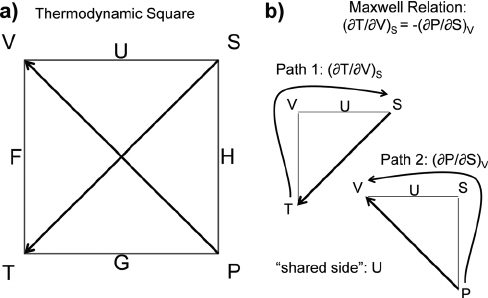
\includegraphics[scale=0.33]{Images/maxwell-square.png}
    \caption{Maxwell mnemonic square with an example.}
    \label{fig:maxwell}
\end{figure}

\newpage
\textbf{Procedure for Derivative Reduction:}

\begin{enumerate}
    \item If the derivative contains any potentials, bring them one by one to the numerator and eliminate by the thermodynamic square. ($dU=TdS-PdV+\mu dN$)
    \item If the derivative contains the chemical potential, bring it to the numerator and eliminate by means of the Gibbs-Duhem relation, $d\mu = -s dT + v dP$
    \item If the derivative contains the entropy, bring it to the numerator. If one of the four Maxwell relations of the thermodynamic square now eliminates entropy, invoke it. If not, then put a $\partial T$ under $\partial S$. The numerator will then be expressible as one of the specific heats ($c_v,c_p$).
    \item Bring the volume to the numerator. The remaining derivative will be expressible in terms of $\alpha$ and $\kappa_T$.\footnote{I have added a \hyperref[subsec::partials]{section} with information from Appendix A of Callen that describes the derivative reduction mathematically.}
    \item The originally given derivative has now been expressed in terms of the four quantities $c_v,c_p,\alpha,$ and $\kappa_T$. The specific heat at constant volume is eliminated by equation:
    \[
    c_v = c_p -Tv\alpha^2/\kappa_T
    \]
\end{enumerate}


I find this figure of an example from Wikipedia helpful.
\begin{figure}[!h]
    \centering
    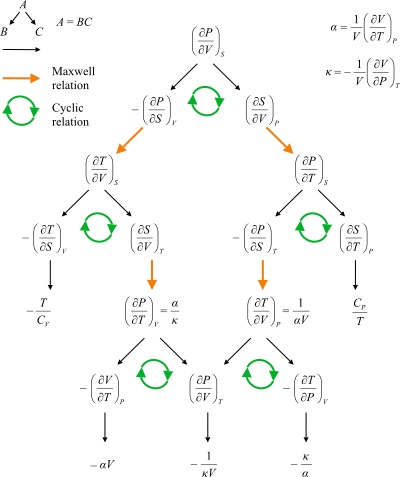
\includegraphics[scale=0.48]{Images/thermo-flow.png}
    \caption{Flow chart for thermodynamic relations.}
    \label{fig:derivflow}
\end{figure}
\section{Grand-Canonical Formalism}

\emph{Kittel \& Kroemer: Chapter 5}
\begin{itemize}
    \item Know the Gibbs Sum \& Gibbs Factor
    \item Use thermal, chemical reservoir
    \item Construct Grand-Canonical partition function and compute expectation values
\end{itemize}

The Grand-Canonical Formalism is used to describe the states of a system in equilibrium with a thermal and chemical reservoir. The same arguments from the Canonical Formalism carries over.

\textbf{Gibbs Factor:} Gives the relative probability of a state $s$ with occupation $N_s$ and energy $\epsilon_s$ by
\[
\exp{[(N_s\mu-\epsilon_s)/\tau]}
\]

\textbf{Gibbs Sum:} (OR Grand-Canonical Partition Function) sums all of the Gibbs Factor so one can calculate the absolute probability of a given state.
\[
\mathcal{Z} = \sum_{all} \exp{[(N_s\mu-\epsilon_s)/\tau]}
\]
This gives the probability as
\[
\mathbb{P}(x) = \frac{e^{(N_x\mu-\epsilon_x)/\tau}}{\sum_{all} e^{(N_s\mu-\epsilon_s)/\tau}}
\]
The expectation values are calculated in the usual way.

\textbf{Absolute Activity:} Sometimes useful to use this lambda notation.
\[
\lambda \equiv e^{\mu/\tau}
\]
\section{Fermi-Dirac \& Bose-Einstein Distributions}

\emph{Kittel \& Kroemer: Chapter 6}
\begin{itemize}
    \item How to construct from Grand Canonical Formalism
    \item Will be given distribution, energy function, Fermi energy, etc. if needed
\end{itemize}
NOTE: Both distributions tend towards the same result in the high $\tau$ limit. This describes an "ideal gas", and it is the \textbf{Classical Distribution Function:}
\[
f(\epsilon) \approx e^{(\mu-\epsilon)/\tau} = \lambda e^{-\epsilon/\tau}
\]
\subsection{Fermi-Dirac Distribution}

Describes the distribution of fermions over energy states in a system. Fermions are 1/2 integer spin and obey Pauli Exclusion Principle (Either 0 or 1 particle occupying each state). The expectation value of the "Thermal Average Occupancy" $\langle N(\epsilon) \rangle$ in the Grand-Canonical Formalism gives the \textbf{Fermi-Dirac Distribution:}
\[
\langle N(\epsilon) \rangle = f_{FD}(\epsilon) = \frac{1}{e^{(\epsilon - \mu)/\tau}+1}
\]

\textbf{Fermi Level:} $\mu$ in this equation is often referred to by this name in Solid State Physics.

\textbf{Fermi Energy:} $\epsilon_F$ is the highest occupied energy value at $\tau=0$




\subsection{Bose-Einstein Distribution}

Describes the distribution of bosons over energy states in a system. Bosons have integer spin and can occupy the same state without limit. The "Thermal Average Occupancy" $\langle N(\epsilon) \rangle$ in the Grand-Canonical Formalism for bosons gives the \textbf{Bose-Einstein Distribution:}
\[
\langle N(\epsilon) \rangle = f_{BE}(\epsilon) = \frac{1}{e^{(\epsilon - \mu)/\tau}-1}
\]

\section{Degenerate Gas}

\emph{Kittel \& Kroemer: Chapter 7}
\begin{itemize}
    \item Using Fermi-Dirac Distribution in the low temperature limit
    \item How to use zero temperature Fermi-Dirac Distribution to find expectation values
\end{itemize}

Whenever $n \geq n_Q$ the gas is said to be in the quantum regime, which occurs at high density or low temperature. This is when there are more particles than available states at a given temperature. This is often called a \textbf{degenerate gas}\footnote{Otherwise called "zero-temperature gas", "ground state", or simply "fermi gas".}. The applications of this theory include:
\begin{itemize}
    \item conduction electrons in metals\footnote{This is most familiar to people most likely. I work in this area so am a bit biased towards this application.}
    \item white dwarf stars
    \item liquid $^3$He
    \item nuclear matter
    \item phonons in solids
\end{itemize}
I do not like Kittel's treatment very much, but Dr. Townsley gave good notes in lecture. I highly recommend learning about Bose-Einstein condensates from the book or elsewhere since the class did not get to it. This concept is a big deal in some areas of physics (like Cooper pairs in Type I Superconductors).

\textbf{Fermi Energy:} This concept is revisited in this context. The energy of the highest filled orbital in the ground state of a free particle gas of fermions (will be given to us on exam) is
\[
\epsilon_F = \frac{\hbar^2}{2M} \bigg( \frac{3\pi^2N}{V} \bigg)^{2/3}
\]
Which can be used to find the total kinetic energy in the ground state as 
\[
U_0 = \frac{3}{5} N \epsilon_F
\]

\textbf{Fermi Temperature:} $\tau_F = \epsilon_F$

\textbf{Fermi Occupancy:} $n_F$ is the value of $n$ in the expression of $\epsilon_F$
\begin{figure}[!hbtp]
    \centering
    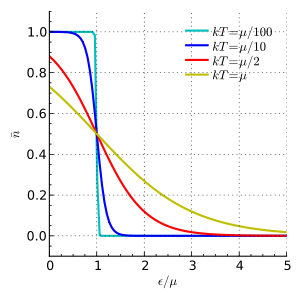
\includegraphics[scale=.2645]{Images/FD-dis.png}
    \caption{Behavior of Fermi-Dirac distribution at different temperatures.}
    \label{fig:fd-dis}
\end{figure}

\newpage
\textbf{Derivation from class:}
The energy of an un-bound electron in a "box" is 
\[
\epsilon_n = \frac{\hbar^2\pi^2}{2mL^2} n^2
\]

We want the Average Occupancy $\langle N \rangle$. This is given by the sum of the Fermi-Dirac Distribution over all energies. This sum can be turned into an integral if the gaps between energy values is small enough, and a factor of two is added for the spin multiplicity.
\[
\langle N \rangle = \int_{all} f_{FD}(\epsilon) d\epsilon 
= 2 \int_0^{\infty} \int_0^{\infty} \int_0^{\infty} f_{FD}(\epsilon) dn_x dn_y dn_z
\]

One can note that the value of $\epsilon$ only depends on the magnitude of $n$, which lends itself to a conversion into pseudo-spherical coordinates in phase space $dn_x dn_y dn_z \to n^2 sin\theta dn d\theta d\phi$. The quantum numbers are only positive, so the limits of integration correspond to the first octant. This is summarized below.
\[
    \left. \begin{aligned}
        0 \leq n_x \\
        0 \leq n_y \\
        0 \leq n_z
    \end{aligned}
    \right \}
\qquad
\implies
    \left. \begin{aligned}
        0 \leq n \\
        0 \leq \theta \leq \pi/2 \\
        0 \leq \phi \leq \pi/2
    \end{aligned}
    \right \}
\]

The figure above shows how the Fermi-Dirac Distribution approaches the behavior of a step function at zero temperature. This can be written as
\[
f_{FD} = \begin{cases}
            1,  n < n_F \\
            0,  n > n_F
         \end{cases}
\]
Which makes the integral
\[
\langle N \rangle = 2 \int_0^{n_F} \int_0^{\pi/2} \int_0^{\pi/2} f_{FD}(\epsilon) n^2 sin\theta dn d\theta d\phi = \frac{\pi}{3} n_F^3 = N
\]
This can be solved for $n_F = (3N/\pi)^{1/3}$ and put into the $\epsilon_F$ to get it in terms of $N,V$.
\[
\epsilon_F = \frac{\hbar^2}{2M} (3\pi^2)^{2/3} \bigg( \frac{N}{V} \bigg)^{2/3}
\]

Now, to get the expectation value for the energy $\langle U \rangle$, a similar procedure is followed.
\[
\langle U \rangle = 2 \int_0^{\infty} \int_0^{\infty} \int_0^{\infty}  \epsilon(n) f_{FD}(\epsilon) dn_x dn_y dn_z
\]
Using the same change of coordinates
\[
\langle U \rangle = 2 \int_0^{n_F} \int_0^{\pi/2} \int_0^{\pi/2}  \epsilon(n) f_{FD}(\epsilon) n^2 sin\theta dn d\theta d\phi = \frac{\pi^3\hbar^2}{10mL^2} n_F^5
\]
Which becomes the final result
\[
U = \frac{3}{5} N \epsilon_F
\]

\newcommand{\diver}{\ensuremath{\nabla \cdot}}
\newcommand{\curl}{\ensuremath{\nabla \times}}
\newcommand{\unitv}[1]{\ensuremath{\mathbf{\hat{#1}}}}
\newcommand{\diff}[2]{\ensuremath{\frac{\partial #1}{\partial #2}}}

\chapter{Griffiths Electrodynamics Review}


\section{Maxwell's Equations}
Dr. Butler recommends reading the Maxwell review on Blackboard (\href{https://ualearn.blackboard.com/bbcswebdav/pid-3974540-dt-content-rid-36341461_1/courses/11111.201910/Reading\%20Assingnments/Review\%20of\%20Maxwell\%27s\%20Equations\%281\%29.pdf}{link}).


\subsection{WHB Pedagogical Transformations}
Dr. Butler does not think the way Griffiths presents Maxwell's equations is the best. Dr. Butler likes to write them in terms of the electric field $\mathbf{E}$ and magnetic field $\mathbf{H}$, and relate these to the electric flux density $\mathbf{D}$ and $\mathbf{B}$ with the polarization $\mathbf{P}$ and magnetization $\mathbf{M}$. They turn into the following

    \begin{align*}
        \diver \mathbf{E} &= \frac{\rho_e}{\epsilon_0} & -\curl \mathbf{E} = \mathbf{J}_m + \diff{\mathbf{B}}{t} \\
        \diver \mathbf{H} &= \frac{\rho_m}{\mu_0} & \curl \mathbf{H} = \mathbf{J}_e + \diff{\mathbf{D}}{t}
    \end{align*}
    
with $\rho_m$ being the "magnetic charge" and $\mathbf{J}_m$ being the "magnetic current." These are related to the flux densities by (Butler's magnetization to Griffiths is: $\mathbf{M}'=\mu_0 \mathbf{M}$)
    \begin{align*}
        \mathbf{D} = \epsilon_0 \mathbf{E} + \mathbf{P} \hspace{20pt}    \mathbf{B} = \mu_0 \mathbf{H} + \mathbf{M}' \\
    \end{align*}
    
\emph{Should know how to transform to Griffiths form.}

\textbf{Charge densities with media:}
    \begin{align*}
        \diver \mathbf{D} &=  \epsilon_0 \diver \mathbf{E} + \diver \mathbf{P} & \diver \mathbf{B} &= \mu_0 \diver \mathbf{H} + \diver \mathbf{M}' \\
        \rho_{ef} &= \rho_e - \rho_{eb} & \rho_{mf} &= \rho_m - \rho_{mb} 
    \end{align*}
    
\subsection{Experimental Basis for Maxwell Equations}
Dr. Butler (and many other professors) have emphasized the experimental basis of these equations. He expects us to know them.

\subsubsection{Coulomb's Potentials}
% ADD DERIVATION AND MAYBE DIAGRAM
Coulomb's experiments in the 18th century imply both divergence equations. The experiment measured the proportionality between the fields and the amount of charge for electric charges and magnetic poles. This inverse square relation with a Green's function and the divergence theorem gives the divergence equations.
    \begin{align*}
        \diver \mathbf{E} = \frac{\rho_e}{\epsilon_0} \hspace{20pt} \diver \mathbf{H} = \frac{\rho_m}{\mu_0} \\
    \end{align*}

\begin{figure}[!hbtp]
    \centering
    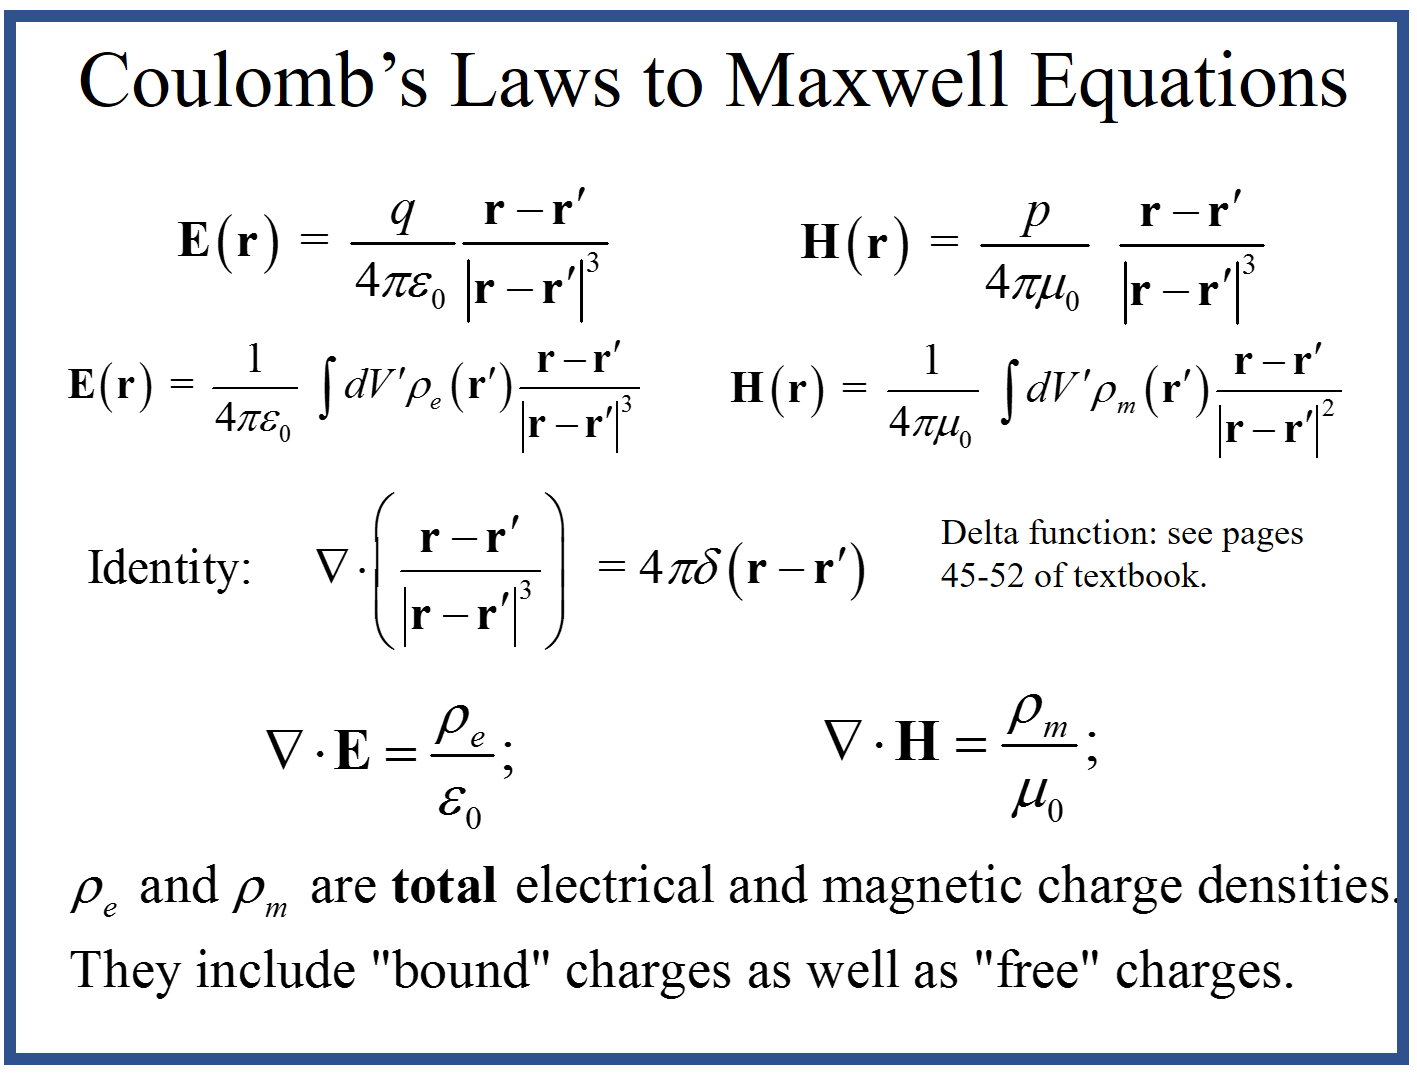
\includegraphics[scale=.2]{Images/coloumb.png}
    \caption{Derivation of Divergence Laws from Coulomb experiments.}
    \label{fig:coulomb}
\end{figure}

\subsubsection{Ampere's Law}
% FILL
Ampere observed 
\textcolor{orange}{UNDER CONSTRUCTION.}


\subsubsection{Maxwell Correction}
% FILL
\textcolor{orange}{UNDER CONSTRUCTION.}


\subsubsection{Faraday's Experiments}
% FILL
\textcolor{orange}{UNDER CONSTRUCTION.}
% W, C, N, m, s preferred

\section{Units of Electromagnetic Quantities}
"If you do not know the units of every symbol in your equation, it is almost meaningless."

\begin{table}[!hbtp]
    \centering
    \caption{Units Table}
    \begin{tabular}{c | c | c}
        \toprule
        Symbol     & Name                  & Standard Units \\
        \toprule
        $\nabla$   & Del operator          & $1/m$          \\
        H          & Magnetic Field        & $N/W$          \\
        B          & Magnetic Flux Density & $W/m^2$        \\
        E          & Electric Field        & $N/C$          \\
        D          & Electric Flux Density & $C/m^2$        \\
        P          & Polarization          & $C/m^2$        \\
        M'         & Magnetization         & $W/m^2$        \\
        $\epsilon$ & Permittivity          & $C/m^2s$      \\
        $\mu$      & Permeability          & $W/m^2s$      \\
        u          & Energy Density        & $J/m^3$       \\
        \bottomrule
    \end{tabular}
    \label{tab:units}
\end{table}

\textbf{Useful conversions:}

\[
\frac{N}{Cm} = \frac{W}{m^2s} \implies \frac{W}{s} = \frac{Nm}{C} = \frac{J}{C} = V
\]
\[
[E] = \frac{W}{sm} \text{  or  } [E] = \frac{V}{m}
\]
And
\[
[H] = \frac{N}{W} \text{  or  } [H] = \frac{A}{m}
\]

\textbf{\textcolor{red}{Memorize:}}
\[
J = A \cdot W
\]

\section{Conservation in Electrodynamics}

\emph{Noether's Theorem} states, \emph{If there is a conservation law, the action is stationary under an infinitesimal transformation in an appropriate variable.} Which can be stated as the converse, \emph{If the action is stationary under an infinitesimal transformation, there is a corresponding conservation law.}\footnote{Schwinger et al. \emph{Classical Electrodynamics}}

\begin{table}[!hbtp]
    \centering
    \begin{tabular}{c c}
        \toprule
        Transformed Variable  &  Conserved Quantity \\
        \toprule
        Time                  &  Energy             \\
        Space                 &  Momentum           \\
        Rotation              &  Angular Momentum   \\
        Gauge change          &  Charge             \\
    \end{tabular}
    \caption{A table of conserved quantities and the variable that implies them. The left column is the variable undergoing an infinitesimal transformation, and the right column is the implied conservation law.}
    \label{tab:conserve}
\end{table}

%\subsection{Conservation of Charge}
% FILL
% Div J = -d rho /dt


\subsection{Conservation of Energy}
This is a very consequential element of Griffiths' treatment of electrodynamics. The Energy for Electrostatics and Magnetostatics have been derived to be:\footnote{Note that these integrals are over all space, not the charge distribution.}

\begin{align*}
    W_e &= \frac{\epsilon_0}{2} \int E^2 d\tau \\
    W_m &= \frac{\mu_0}{2} \int H^2 d\tau
\end{align*}

The energy density can be written in two ways in vacuum:

\[
u = \frac{1}{2} \Big( \epsilon_0 E^2 + \frac{1}{\mu_0} B^2 \Big)  \text{    OR    } u = \frac{1}{2} \Big( \epsilon_0 E^2 + \mu_0 H^2 \Big)
\]
and in \emph{linear} media it becomes:
\[
u = \frac{1}{2} \Big( \textbf{E} \cdot \textbf{D} + \textbf{H} \cdot \textbf{B} \Big)
\]


\newpage




\chapter{Theory of Probability}

These are the essentials of the Theory of Probability (MATH 355) class taught by Dr. Beznosova in Spring 2019.


\section{Foundations of Probability}

\subsection{Principle Definitions}
Some terms that are needed to build the foundations are defined below.
\begin{itemize}
    \item \textbf{Sample space} S is a set that includes all possible outcomes of a random experiment listed in a mutually exclusive and exhaustive way.
    \item \textbf{Mutually exclusive} means that outcomes of the set do not overlap.
    \item \textbf{Exhaustive} means that the list contains all possible outcomes.
    \item \textbf{Event} is a set of outcomes that is a subset of the sample space.
\end{itemize}

\subsection{Venn Diagrams and Set Theory}

\begin{figure}[!hbtp]
    \centering
    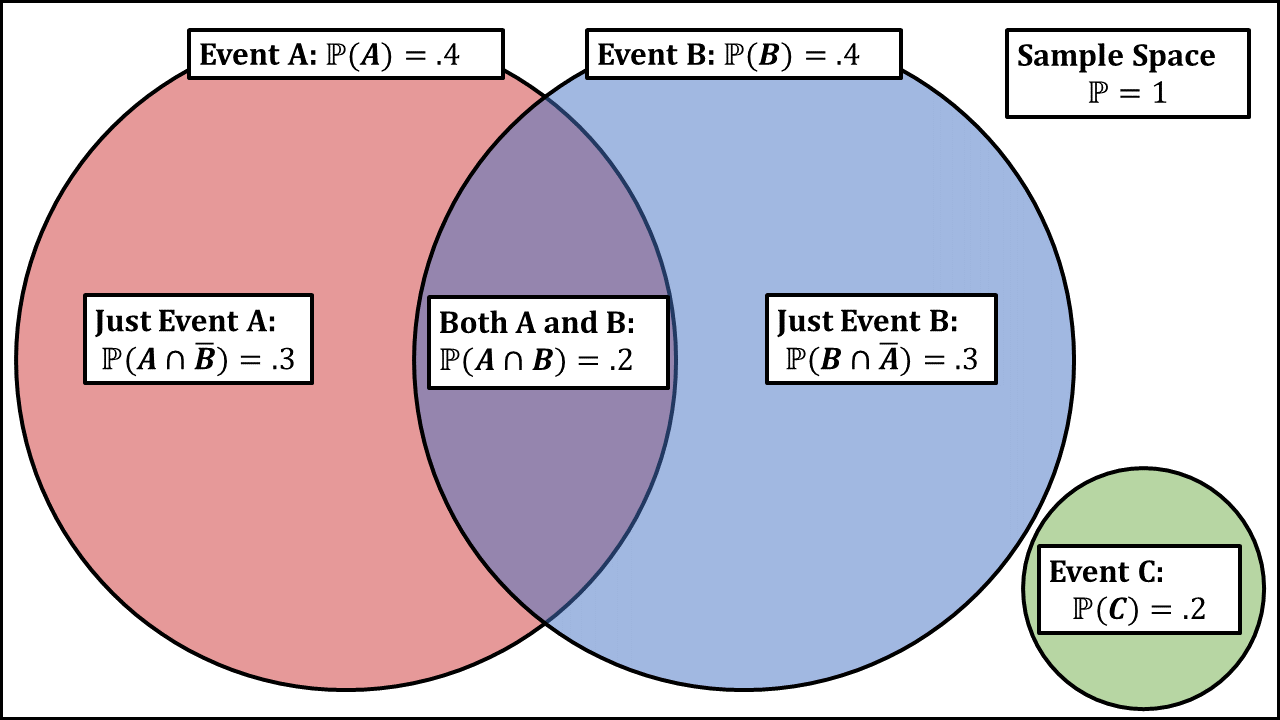
\includegraphics[scale=.3]{Images/venndiagram.PNG}
    \caption{An example of a sample space being represented by a venn diagram.}
    \label{fig:venndiagram}
\end{figure}
\input{355Review/section_conditional.tex}
\input{355Review/section_discrete.tex}
\input{355Review/section_continuous.tex}
\input{355Review/section_multivariate.tex}


\newpage
\renewcommand\thesubsection{\Alph{subsection}}

\phantomsection
\addcontentsline{toc}{section}{Math Appendix}
\section*{Math Appendix}


\subsection{Partial Derivative Relations}
\label{subsec::partials}

If you, like myself, find the derivative reduction process confusing, then I recommend reading the section in Appendix A of Callen called "Some Relations Involving Partial Derivatives." I summarize with the most useful relations below.

Begin with general function $\psi(x,y,z)$, and you can use the following relations between the partial derivatives:

\[
    \bigg(\frac{\partial y}{\partial x} \bigg)_{\psi,z} = \frac{-\Big(\frac{\partial \psi}{\partial x}\Big)_{y,z}} {\Big(\frac{\partial \psi}{\partial y}\Big)_{x,z}}   
\]
With similar expressions for the partials in the other derivatives. This is used to bring variable (usually S) out of the constants.

\[
    \bigg(\frac{\partial x}{\partial y} \bigg)_{\psi,z} = \frac{1} {\Big(\frac{\partial y}{\partial x}\Big)_{\psi,z}} 
\]
This one is the most elementary looking, and it is usually used to bring S or V to the numerator.

\[
    \bigg(\frac{\partial y}{\partial x} \bigg)_{\psi,z} = \frac{\Big(\frac{\partial y}{\partial u}\Big)_{\psi,z}} {\Big(\frac{\partial x}{\partial u}\Big)_{\psi,z}}
\]
Can be used to put T into the derivatives when using the standard set of derivatives.

\end{document}
